%KECReportFormat.tex
%%%%%%%%%%%%%%%%%%%%%%%%%%%%%%%%%%%%%%%%%%%%%%%%%%%%%%%%%%%%%%%%%%%%%%%%%%%
%DO NOT MAKE CHANGES IN THIS FILE

\documentclass[12pt, a4paper]{report}
\usepackage[left = 1.5in, right = 1in, top = 1in, bottom = 1in]{geometry}%for margin
\usepackage{amsfonts, amsmath, amssymb} %for mathematical equations
\usepackage{graphicx} %for images
\usepackage{times} %font Times New Roman Font
\usepackage{float} %required if you use H(strictly here) position for floats
\usepackage[skip = 8pt,tableposition=top, figureposition=bottom]{caption}%adjust spacing of captions and specify where captions are
\usepackage{hyperref} % for easy Navigation in document, also puts links in TOC, LOF, LOT...
\usepackage{setspace} %to change line spacing in some portion \singlespacing \onehalfspacing \doublespacing
\usepackage{acro} %for List of Abbrreviation and Symbol
\acsetup{first-style = short} % set to display only short form on the command \ac{}

%packages required for complex tables
\usepackage{bigstrut} 
\usepackage{multirow}

\renewcommand{\contentsname}{Table of Contents} %Change TOC Heading ... default is "Contents" 

\parindent 0pt	%removes the indent in paragraph
\setlength{\parskip}{18pt}	%for paragraph spacing
\renewcommand{\baselinestretch}{1.5}   %Line Spacing = 1.5 line-spaces

%to reduce spacing in sections
\usepackage{titlesec}
\titlespacing*{\section}{0pt}{0pt}{0pt} %left, top, bottom spacings
\titlespacing*{\subsection}{0pt}{0pt}{0pt}
\titlespacing*{\subsubsection}{0pt}{0pt}{0pt}
\titlespacing*{\paragraph}{0pt}{0pt}{0pt}
\titlespacing*{\subparagraph}{0pt}{0pt}{0pt}

%adjust fontsizes\ of sections
\titleformat*{\section}{\fontsize{14pt}{18pt}\bfseries}
\titleformat*{\subsection}{\fontsize{13pt}{18pt}\bfseries}
\titleformat*{\subsubsection}{\fontsize{12pt}{18pt}\bfseries}
\titleformat*{\paragraph}{\fontsize{12pt}{18pt}\bfseries}
\titleformat*{\subparagraph}{\fontsize{12pt}{18pt}\bfseries}

%to reduce separation between points in list
\usepackage{enumitem}
\setlist[enumerate]{nosep} % no separation between items in enumerate
\setlist[itemize]{nosep} % no separation between items in itemize
%use \vspace{-18pt} before list to reduce paragraph spacing between list and preceeding paragraph.

%Changes for Chapter Heading Spacing and formats for numbered chapters
\makeatletter
\def\@makechapterhead#1{%
  %\vspace*{50pt}%
  {  \MakeUppercase{\ifnum \c@secnumdepth >\m@ne
        \fontsize{16pt}{1}\bfseries \@chapapp \space \thechapter\vspace{5pt}\\
    \fi
    \interlinepenalty\@M
     \bfseries #1}\par\nobreak
    %\vskip 0pt
  }}
\makeatother

%%%%%%%%%%%%%%%%%%%%%%%%%%%%%%%%%%%%%%%%%%%%%%%%%%%%%%%%%%%
%to adjust Heading spacings and fonts For unnumbered chapters, TOC, LOF ...
\makeatletter
% Redefine the \chapter* header macro to remove vertical space
\def\@makeschapterhead#1{%
  %\vspace*{50\p@}% Remove the vertical space
  {\newpage \parindent \z@ \raggedright
    \normalfont
    \interlinepenalty\@M
    \center \fontsize{16pt}{1} \bfseries \MakeUppercase{#1}\par\nobreak
    %\vskip 18\p@ % adjust space after heading 18pt
  }}
\makeatother 
%%%%%%%%%%%%%%%%%%%%%%%%%%%%%%%%%%%%%%%%%%%%%%%%%%%%%%%%%%%

%%%%%%%%%%%%%%%%%%%%%%%%%%%%%%%%%%%%%%%%%%%%%%%%%%%%%%%%%%%%%%%%%%%%%%%%%%%
% newcommand for generating Cover Page
\newcommand{\KECcoverpage}
{
\begin{titlepage}
\begin{center}
\Large{\textbf{KANTIPUR ENGINEERING COLLEGE}}\\
\large{\textbf{(Affiliated to Tribhuvan University)}}\\
\large{\textbf{Dhapakhel, Lalitpur}}\\
\vfill	%vertically fill the space 
\begin{figure}[h] % h: put logo "here"
\begin{center}

\includegraphics[width=25mm, height = 25mm]{images/logo.png}
\end{center}
\end{figure}

\large{\textbf{[Subject Code: \subCode]}}\\ %Change This Line
\large{\textbf{A \MakeUppercase{\project} \MakeUppercase{\doc} ON}}\\ %Change This Line
\Large{\textbf{\MakeUppercase{\projectTitle}}}\\

\vfill	%vertically fill the space 
\large{\textbf{Submitted by:}}\\
\large{\textbf{\submittedBy}}\\
\vfill	%vertically fill the space 
\textbf{A \MakeUppercase{\project} SUBMITTED IN PARTIAL FULFILLMENT OF THE REQUIREMENT FOR THE DEGREE OF \MakeUppercase{\degree}}\\

\vfill	%vertically fill the space 
\large{\textbf{Submitted to:}}\\
\large{\textbf{\submittedTo}}\\
\vfill
\large{\textbf{\defMonth, \defYear}}
\pagebreak
\end{center}
\end{titlepage}
}
%%%%%%%%%%%%%%%%%%%%%%%%%%%%%%%%%%%%%%%%%%%%%%%%%%%%%%%%%%%%%%%%%%%%%%%
% newcommand for generating Cover Page
%Title Page
\newcommand{\KECtitlepage}
{
\begin{titlepage}
\begin{center}
\Large{\textbf{\MakeUppercase{\projectTitle}}}\\

\vfill	%vertically fill the space 

\large{\textbf{Submitted by:}}\\
\large{\textbf{\submittedBy}}\\


\ifhassupervisor % Displays Supervisor name only if \hassupervisortrue
	\vfill	%vertically fill the space 
	\large{\textbf{Supervised by:}}\\
	\large{\textbf{\supervisor}}\\
	\large{\textbf{\degSup}}\\
\fi

\vfill	%vertically fill the space 
\textbf{A \MakeUppercase{\project} SUBMITTED IN PARTIAL FULFILLMENT OF THE REQUIREMENT FOR THE DEGREE OF \MakeUppercase{\degree}}\\

\vfill	%vertically fill the space 
\large{\textbf{Submitted to:}}\\
\large{\textbf{\submittedTo}}\\
\large{\textbf{Kantipur Engineering College}}\\
\large{\textbf{Dhapakhel, Lalitpur}}\\

\vfill
\large{\textbf{\defMonth, \defYear}}
\thispagestyle{empty}\\ %to remove page number
\pagebreak
\end{center}
\end{titlepage}
}
%%%%%%%%%%%%%%%%%%%%%%%%%%%%%%%%%%%%%%%%%%%%%%%%%%%%%%%%%%%%%%%%%%%%%%
%command for copyright page
\newcommand{\KECcopyright}
{
\chapter*{Copyright}%Required only for Final Defense of Major Project
\addcontentsline{toc}{chapter}{Copyright}
The author has agreed that the library, Kantipur Engineering Collage, may make this report freely available for inspection. Moreover the author has agreed that permission for extensive copying of this report for scholarly purpose may be granted by the supervisor(s), who supervised the project work recorded herein or, in their absence, by the Head of the Department wherein this project was done. It is understood that due recognition will be given to the author of this report and to the \submittedTo, Kantipur Engineering College in any use of the material of this report. Copying or publication or other use of this report for financial gain without approval of the \submittedTo, Kantipur Engineering College and author’s written permission is prohibited.\par Request for permission to copy or to make any other use of the material in this report in whole or in part should be addressed to:

Head\\
\submittedTo\\
Kantipur Engineering College\\
Dhapakhel, Lalitpur\\
Nepal
}
%%%%%%%%%%%%%%%%%%%%%%%%%%%%%%%%%%%%%%%%%%%%%%%%%%%%%%%%%%%%%%%%%%%%%%
%command for Approval Letter
\newcommand{\KECapproval}
{
\chapter*{Kantipur Engineering College
\vskip -10pt}%Required only for Final Defense of Major Project
\begin{center}
\fontsize{12.8pt}{1} %size decreaced to adjust department name in single line
\textbf{
\MakeUppercase{\submittedTo}\\ %for department name
}
\vskip 10pt
\fontsize{16pt}{1}
\textbf{APPROVAL LETTER}
\end{center}
\vskip -16pt
\addcontentsline{toc}{chapter}{Approval Letter}%
The undersigned certify that they have read and recommended to the Institute of Engineering for acceptance, a project report entitled "\projectTitle " submitted by \\
\submittedBy \\
in partial fulfillment for the degree of \degree. \par
{\vspace{25pt}
..........................................\\
Supervisor\\
\supervisor \\
\degSup\\
\vspace{25pt}\\
..........................................\\
External Examiner\\
\external\\
\degExternal\\
\vspace{25pt}\\
..........................................\\
\hod\\
Head of Department\\
\submittedTo
\vspace{10pt}\\
Date: \defMonth\space\defDay ,\space \defYear
\singlespacing\par
} %single spacing for the texts inside {}
}

%command for list of abbreviations
\newcommand{\KECloa}
{
\chapter*{List of Abbreviations}
\addcontentsline{toc}{chapter}{List of Abbreviations}
\vskip -42pt % to reduce space due to invisivle acronym class name
{
\singlespacing
\printacronyms[include-classes=abbr, name= ]
}

}

%command for list of symbols
\newcommand{\KEClos}
{
\chapter*{List of Symbols}
\addcontentsline{toc}{chapter}{List of Symbols}
\vskip -42pt % to reduce space due to invisivle acronym class name{
{
\singlespacing
\printacronyms[include-classes=symbol, name= ]
}
}

%command to adjust toc, lof, lot spacing
\newcommand{\KECadjusttocspacings}
{
\parskip 0pt % to remove paragraph spacing in TOC, LOF ...
\renewcommand{\baselinestretch}{0.1} % to adjust line spacing in toc
\newcommand*{\noaddvspace}{\renewcommand*{\addvspace}[1]{}}
\addtocontents{lof}{\protect\noaddvspace} %remove extra vertical space in LOF
\addtocontents{lot}{\protect\noaddvspace} %remove extra vertical space in LOT
} %includes the file KecReportFormat.tex that include all necessary formattings
%%%%%%%%%%%%%%%%%%%%%%%%%%%%%%%%%%%%%%%%%%%%%%%%%%%%%%%%%%%%%%%%%%%%%%%%%%%
%Define Macros for Details of your Project
\newcommand{\project}{Major Project} %Specify "Major Project" or "Minor Project"
\newcommand{\projectTitle}{Network Intrusion Detection System Using LSTM} %specify "Title" of Your Project
\newcommand{\doc}{Final Report} % specify the document you are preparing eg. "Proposal", "Mid-Term Report" or "Final Report" 
% Note that You have to sibmit "Final Report" for Pre-final defense as well.
\newcommand{\subCode}{CT755} %specify Subject of Your Project
\newcommand{\degree}{Bachelor in Computer Engineering} %specify your degree
\newcommand{\submittedBy}%Specify Names and Roll/Symbol Numbers of the Project Group Members
{
%Edit Member Names and Roll/Symbol No. and adjust width (\makebox[width]) if necessary 
\makebox[7cm]{Aman Devkota  \hfill[KAN076BCT010]}\\
\makebox[7cm]{Ankur Karmacharya  \hfill[KAN076BCT013]}\\
\makebox[7cm]{Prashad Adhikary  \hfill[KAN076BCT056]}
%\makebox[9cm]{Member Name \hfill [Roll/Symbol No.]}\\
} % Note that You must write your "Symbol Numbers"(Exam Roll Numbers) for Final Defenses

\newcommand{\submittedTo}{Department of Computer and Electronics Engineering} %specify your department
\newcommand{\hod}{Er. Rabindra Khati} %specify Head ot the department
\newcommand{\defYear}{2024} %Defense Year
\newcommand{\defMonth}{March} %Defense Month- January, February, ...
\newcommand{\defDay}{4} %specify Defense Day- 1, 2, ...

\newif\ifhassupervisor
\hassupervisortrue % to display supervisor name use command- \hassupervisortrue
\newcommand{\supervisor}{Dr. Babu Ram Dawadi} % Specify Name of Supervisor for Major Project (write "none" if no Supervisor is assigned)
\newcommand{\degSup}{Asst. Professor\\Department of Electronics and Computer Engineering, IOE\\Pulchowk} %Specify Designation of Supervisor for Major Project, use multiple lines (\\) if necessary
\newcommand{\external}{External's Name} %Specify Name of External for Major Project (Required for Black Book)
\newcommand{\degExternal}{External's Designation\\Second Line of Designation (if required)} %Specify Name of External for Major Project (Required for Black Book) , use multiple lines (\\) if necessary
%%%%%%%%%%%%%%%%%%%%%%%%%%%%%%%%%%%%%%%%%%%%%%%%%%%%%%%%%%%%%%%%%%%%%%%%%%%

%%%%%%%%%%%%%%%%%%%%%%%%%%%%%%%%%%%%%%%%%%%%%%%%%%%%%%%%%%%%%%%%%%%%%%%%%%%

%%%%%%%%%%%%%%%%%%%%%%%%%%%%%%%%%%%%%%%%%%%%%%%%%%%%%%%%%%%%%%%%%%%%%%%%%%%%%%%%%%%%%%%%%%%%%%%%%%%%

%%%%%%%%%%%%%%%%%%%%%%%%%%%%%%%%%%%%%%%%%%%%%%%%%%%%%%%%%%%%%%%%%%%%%%%%%%
%The Document
\setcounter{tocdepth}{3}
\setcounter{secnumdepth}{3}
\begin{document}

\KECcoverpage  
\KECtitlepage
\pagenumbering{roman} % starts pagenumberins in Roman numerals i, ii, ...

%Copyright Page is required for FINAL REPORT only. Comment this section for other Reports.
%\KECcopyright % defined in KECReportFormat.tex

%Approval Page is required for FINAL(Black Book Binded) REPORT of MAJOR PROJECT only. Comment this section for other Reports. 
%\KECapproval % defined in KECReportFormat.tex

\chapter*{Abstract} % The summary of your report
\addcontentsline{toc}{chapter}{Abstract}%to include %this chapter in TOC 
Network intrusion attacks have significantly increased in recent years, which creates serious privacy and security concerns. Technology development has made cyber-security threats more sophisticated, to the point where the detection mechanisms in place are unable to handle the problem. Therefore, the key to solving this issue would be the deployment of a clever and efficient network intrusion detection system. In order to create an intelligent detection system that can recognize many types of network intrusions, we are using deep learning technique in this project, namely Long Short-Term Memory. One of the most recent realistic dataset, InSDN datasets, was used for training and evaluation in order to demonstrate the effectiveness of the suggested system. To evaluate the model, we have used evaluation metrics like accuracy, precision, True Positive Rate, False Positive Rate.
\par
\textbf{\textit{Keywords$-$}} \emph{LSTM,Network Intrusion Detection System (NIDS), InSDN dataset}

\chapter*{Acknowledgment}
\addcontentsline{toc}{chapter}{Acknowledgment}%to include this chapter in TOC
This project is prepeared in partial fulfillment of the requirement for the bachelor's degree in Computer Engineering. We are very grateful to Prof. Dr. Babu Ram Dawadi, our supervisor for guiding us throughout this major project. We would like to express our sincere gratitude to Department head Er. Rabindra Khati, Project Co-ordinator Er. Bishal Thapa and all the faculty members of Kantipur Engineering College for the continuous support during this project for their patience, motivation,enthusiasm, and immense knowledge. Their guidance helped us in all time of research, development and implementation of this project.\par
Finally we would like to thank our family and friends for all the support and encouragement for the completion of this project.\par
%to display members name under Acknowledgement
\begin{flushright}
\vskip -20pt
\setstretch{1.2}
\submittedBy

\end{flushright}

%to adjust spacings for TOC, LOF, LOT
{
%%%%%%%%%%%%%%%%%%%%%%%%%%%%%%%%%%%%%%%%%%%%%%%%%%%%%%%%%%%%%%%%%%%%%%%%%%%
%TOC, LOF and LOT
\KECadjusttocspacings % defined in KECReportFormat.tex to adjust spacings
\makeatletter
% to add vskip of 18 point which is reduced when parskip is set to 0 in \LECadjustspacings
\def\@makeschapterhead#1{%
  %\vspace*{50\p@}% Remove the vertical space
  {\newpage \parindent \z@ \raggedright
    \normalfont
    \interlinepenalty\@M
    \center \fontsize{16pt}{1} \bfseries \MakeUppercase{#1}\par\nobreak
   % \vskip 18\p@ % adjust space after heading 18pt
  }}
\makeatother 

\tableofcontents % prints table of contents
\listoffigures % prints list of figures
\addcontentsline{toc}{chapter}{List of Figures}
\listoftables % prints list of table
\addcontentsline{toc}{chapter}{List of Tables}
}
%%%%%%%%%%%%%%%%%%%%%%%%%%%%%%%%%%%%%%%%%%%%%%%%%%%%%%%%%%%%%%%%%%%%%%%%%%%
\chapter*{List of Abbreviations}
\textbf{DOS}: Denial of Service\\
\textbf{FN}: False  Negative \\
\textbf{FP}: False Positive\\
\textbf{IDS}: Intrusion Detection System\\
\textbf{LSTM}: Long Short-Term Memory\\
\textbf{RFC}: Random Forest Classifier\\
\textbf{RFE}: Recursive Feature Elimination\\
\textbf{R2L}: Root to Local \\
\textbf{SDN}: Software Defined Networking \\
\textbf{TN}: True Negative\\
\textbf{TP}: True Positive\\
\textbf{U2R}: User to Root\\
\addcontentsline{toc}{chapter}{List of Abbreviations}
%comment this chapter if you don't have List of Abbreviations
%\KECloa % defined in KECReportFormat

%comment this chapter if you don't have List of Symbols
%\KEClos % defined in KECReportFormat

\newpage
\pagenumbering{arabic} % starts pagenumbering in arabic numerals

\chapter{Introduction}
\vspace{-18pt}
\section{Background}\label{sec:bkgrnd}%label your section if you require to refer them somewhere else in your document.
\vspace{-18pt}
%nw3
With the increasingly deep integration of the Internet and society, the Internet is changing the way in which people live, study and work, but the various security threats that we face are becoming more and more serious. How to identify various network attacks, especially unforeseen attacks, is an unavoidable key technical issue. An Intrusion Detection System, a significant research achievement in the information security field, can identify an invasion, which could be an ongoing invasion or an intrusion that has already occurred. In fact, intrusion detection is usually equivalent to a classification problem, such as a binary or a multi class classification problem, i.e., identifying whether network traffic behavior is normal or anomalous, or a five-category classification problem, i.e., identifying whether it is normal or any one of the other four attack types: DOS, U2R, Probe (Probing) and Root to Local. In short, the main motivation of intrusion detection is to improve the accuracy of classifiers in effectively identifying the intrusive behavior.\par
Machine learning methodologies have been widely used in identifying various types of attacks, and a machine learning approach can help the network administrator take the corresponding measures for preventing intrusions. However, most of the traditional machine learning methodologies belong to shallow learning and often emphasize feature engineering and selection; they cannot effectively solve the massive intrusion data classification problem that arises in the face of a real network application environment. With the dynamic growth of data sets, multiple classification tasks will lead to decreased accuracy. In addition, shallow learning is unsuited to intelligent analysis and the forecasting requirements of high-dimensional learning with massive data. In contrast, deep learners have the potential to extract better representations from the data to create much better models. As a result, intrusion detection technology has experienced rapid development after falling into a relatively slow period\cite{yin2017deep}.%chinese
\par
A well-known method of securing the network is through implementing an Intrusion Detection System. IDS was originally implemented in 1980. The main aim of their work was to introduce a mechanism which differentiates between benign activities from malicious ones. Further research was carried out to optimizing this methodology to aid monitoring the network traffic in case of attacks, this system is now known as Network Intrusion Detection System. In NIDS, the detection system is inspecting the incoming and outgoing network traffic from all hosts in real time and based on certain criteria, it can detect and identify the attack, then, take the suitable security measures to stop or block it, which significantly reduces the risk of damage to the network. However, due to the rapid increase in the complexity of the cyber-security attacks, the current methods used in NIDS are failing to sufficiently address this issue\cite{al2020using}.
\par 
IDSs can be divided into two categories according to the main detection technology: misuse detection and anomaly detection. Misuse detection is a knowledge-based detection technology. A misuse detection system needs to clearly define the features of the intrusion, then identify the intrusion by matching the rules. Misuse detection can achieve a high accuracy and low false alarm rate. However, it needs to build a feature library and cannot detect unknown attacks. In contrast, anomaly detection is a behavior-based detection technology. First, it needs to define the normal activities of a network, and then check whether the actual behavior has deviated from the normal activities. Anomaly detection needs only to define a normal state of a specific network, without prior knowledge of intrusion. Thus, it can detect unknown attacks, although there may be a high false alarm rate. At present, network structure is becoming more and more complicated, and intrusion methods are following the trend of diversification and complication, creating more challenges for IDSs.\par 
The RNN has failed to become a mainstream network model in the past few years due to difficulties in training and computational complexity. In recent years, with the development of deep learning theory, RNN began to enter a rapid development period. Currently, RNN has already been applied successfully to handwriting and speech recognition. The main feature of RNN is that it circulates information in a hidden layer which can remember information processed previously, leading to a structural advantage for the processing of time series information. Correspondingly, many intrusion behaviors can be abstracted as specific time series of events from the underlying network. So, RNN is considered suitable for building an IDS\cite{xu2018intrusion}.
\par 
\section{Problem Statement}
\vspace{-18pt}
The existing Network Intrusion Detection Systems face challenges in accurately and efficiently detecting and preventing network intrusions, thereby compromising the overall security of computer networks. These challenges include high false-positive rates, limited scalability, inability to detect novel or sophisticated attacks, and the difficulty in distinguishing between legitimate and malicious network traffic. Addressing these issues is crucial to enhance the performance and reliability of NIDS, enabling proactive identification and prevention of network intrusions while minimizing false alarms.
\section{Objectives}
\vspace{-18pt}
The primary objective of this project:
\vspace{-18pt}
\begin{enumerate}[label=\roman*.]
\item To develop a robust and accurate system that can effectively detect network intrusions within a computer network.
\end{enumerate}
\section{Project Features}
\vspace{-18pt}
The project will be able to accomplish following:
\vspace{-18pt}
\begin{itemize}
\item Anomaly Detection
\item Traffic Preprocessing
\end{itemize}
\section{Application Scope}
\vspace{-18pt}
Network Intrusion Detection System has various applications in areas such as Enterprise networks, Internet Service Providers, Cloud Computing environment, Government networks and so on. The application scope of network intrusion detection systems using deep neural networks extends beyond these areas, as network security is crucial in nearly every sector that relies on secure and reliable communication. By deploying these systems, organizations can proactively detect and respond to network intrusions, minimize the impact of attacks, and protect their assets, data, and operations from potential threats.
\section{System Requirement}
\vspace{-18pt}
\subsection{Development Requirements}
\vspace{-18pt}
\subsubsection{Software Requirements}
\vspace{-10pt}
\begin{itemize} 
\item Windows/Linux/Mac
\item VMware/Virtualbox
\item Mininet, POX controller
\item Jupyter Notebook
\item Python IDE
\end{itemize}
\subsubsection{Hardware Requirements}
\vspace{-10pt}
\begin{itemize}
\item PC with at least 4-8 GB RAM
\item  Higher graphics of at least 2 GB
\end{itemize}
\subsection{Deployment Requirements}
\vspace{-18pt}
\subsubsection{Software Requirements}
\vspace{-10pt}
\begin{itemize}
\item Windows/Linux/Mac
\item VMware/Virtualbox
\item Mininet, POX controller
\end{itemize}
\vspace{-10pt}
\subsubsection{Hardware Requirements}
\vspace{-10pt}
\begin{itemize}
\item More than 1.5 GHz clock speed
\item Minimum 4 GB RAM
\end{itemize}
\label{tblSampleTable}
%\end{table}
\section{Project Feasibility}
\vspace{-18pt}
\subsection{Technical Feasibility}
\vspace{-18pt}
The technical feasibility assessment is focused on gaining in understanding of the present technical resources required by the system and their applicability to the expected needs of the proposed system. Regarding the proposed system, the technical requirement includes a PC.
\vspace{-18pt}
\subsection{Operational Feasibility}
\vspace{-18pt}
The user will not need any formal knowledge about programming so our project is operationally feasible.
\vspace{-18pt}
\subsection{Economic Feasibility}
\vspace{-18pt}
The purpose of the economic feasibility assessment is to determine the positive economic benefits to the user that the proposed system will provide. Most of the software used for the development is free. Thus, the project is economically feasible.
\vspace{-18pt}
\subsection{Schedule Feasibility}
\begin{figure}[!h] % tbh means top, bottom or here (priority: left to right)
\begin{center}
	%
\includegraphics[width = 3in]{images/logo.png}
	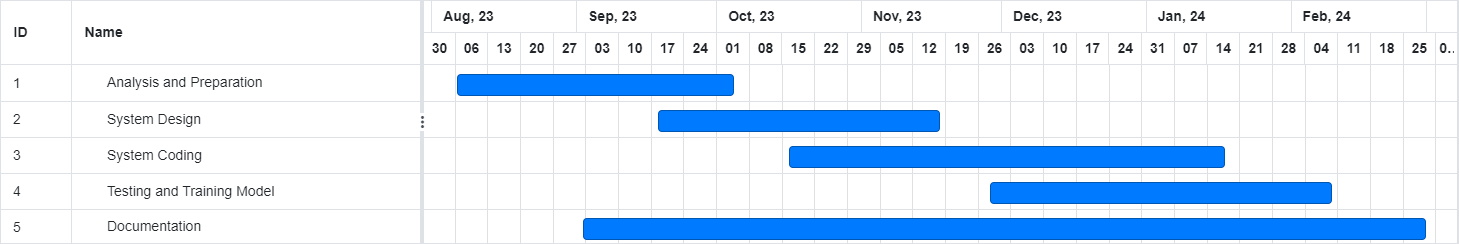
\includegraphics[width=6in,height=2in
	]{images/gn.png} 
	\caption{Gantt Chart} %figure name
	\label{figGanttChart} % for referencing
\end{center}
\end{figure}
\chapter{Literature Review}
\vspace{-18pt}
\section{Related Projects}
\vspace{-18pt}
\subsection{Suricata}
\vspace{-18pt}
Suricata is a leading open-source network analysis and threat detection tool, widely recognized for its high performance and versatility across various platforms including Windows, Mac, Unix, and Linux. Developed by the Open Information Security Foundation, Suricata is embraced by a broad spectrum of users from private and public sectors to major vendors seeking to bolster their cybersecurity defenses. Its utility spans enterprises of all sizes, offering a cost-effective solution for intricate security monitoring needs.\par 
Distinguished by its dual functionality, Suricata serves not only as an intrusion detection system that identifies and alerts on potential threats but also as an intrusion prevention system with capabilities to actively intervene and mitigate identified threats by blocking malicious traffic. This dual capability sets Suricata apart in the cybersecurity domain, enabling comprehensive protection against a wide array of cyber threats.\par 
One of the core strengths of Suricata lies in its sophisticated rule set and signature language, which allows for precise threat detection and prevention strategies. Additionally, its proficiency in deep packet inspection (DPI) further enhances its effectiveness, making it an ideal solution for a variety of security monitoring initiatives. Whether it's for detecting subtle anomalies or preventing advanced cyber attacks, Suricata's robust feature set ensures that organizations can safeguard their digital assets effectively. As a result, Suricata stands out as a versatile and powerful tool in the arsenal of cybersecurity professionals, offering a free yet invaluable resource for securing network environments against the ever-evolving landscape of cyber threats.
\subsection{Snort}
\vspace{-18pt}
Snort stands as the premier Open Source Intrusion Prevention System globally, renowned for its versatility and comprehensive security capabilities. At its core, Snort operates by implementing a robust set of rules designed to identify and define malicious network activities. These rules are crucial for detecting packets that exhibit patterns or behaviors indicative of cyber threats, triggering alerts for users to take action. Moreover, Snort's functionality extends beyond mere detection; it can be configured to operate inline, actively intercepting and blocking malicious packets before they infiltrate the network.\par 
Snort's flexibility allows it to serve multiple roles within the cybersecurity framework. It can function as a packet sniffer, akin to tcpdump, offering detailed insights into network traffic for analysis and troubleshooting purposes. Additionally, it serves as an effective packet logger, providing a valuable tool for network traffic debugging by recording data packets traversing the network. Most prominently, Snort excels as a full-fledged network intrusion prevention system, offering robust protection against a wide array of cyber threats.\par 
Available for both personal and business use, Snort can be easily downloaded and configured to suit various security needs. Its open-source nature not only facilitates widespread access but also encourages continuous improvement and updates from a global community of developers and cybersecurity experts. This collaborative approach ensures that Snort remains at the forefront of intrusion prevention technology, providing an essential layer of defense for networks around the world against the ever-evolving landscape of cyber threats.
\vspace{-10pt}
\section{Related Works}
\vspace{-18pt}
The paper titled "A Deep Learning Approach for Intrusion Detection Using Recurrent Neural Networks" introduces a cutting-edge approach to enhancing the efficacy of Intrusion Detection Systems through the implementation of Recurrent Neural Networks. This innovative methodology diverges from traditional machine learning classification techniques by leveraging the dynamic and temporal processing capabilities inherent in RNNs, which are particularly adept at handling sequence data, thus making them an ideal choice for analyzing network traffic and detecting anomalous patterns indicative of cyber threats.\par
The core of this research revolves around the comparative analysis between RNN-IDS and conventional machine learning methods across both binary and multiclass classification scenarios. The comparison aimed to rigorously evaluate the performance of the deep learning-based model in terms of its accuracy in detecting intrusions within network systems. Notably, the findings from this study illuminated the superior performance of the RNN-IDS model, demonstrating a significant improvement in detection accuracy over its traditional counterparts.\par 
This improvement is attributed to the RNN-IDS model's ability to capture and learn from the temporal dependencies present in network traffic data, a critical aspect that traditional machine learning models often overlook. By effectively utilizing the sequential information within the data, RNN-IDS can offer a more nuanced and comprehensive analysis of potential security threats, leading to a higher accuracy rate in intrusion detection.\par 
Moreover, the success of the RNN-IDS model in outperforming established machine learning techniques not only validates the potential of deep learning approaches in the realm of cyber-security but also paves the way for further research into the development of more sophisticated and effective intrusion detection systems. The study concludes by highlighting the RNN-IDS model as a novel and promising research method, capable of significantly enhancing the accuracy and reliability of intrusion detection efforts, thereby contributing to the advancement of security measures in the face of evolving cyber threats\cite{yin2017deep}.
\par 
The study "Using Deep Learning Techniques for Network Intrusion Detection" delves into the development of an advanced intrusion detection system leveraging the strengths of both Convolutional Neural Networks and Recurrent Neural Networks. This innovative approach aimed to harness the unique capabilities of these deep learning models to enhance the detection of various network intrusions, a critical aspect of maintaining cyber security in the digital age. The evaluation of this intelligent detection system was conducted through a comprehensive analysis utilizing a range of performance metrics, including accuracy, F1 score, recall, and precision. These metrics served as the benchmarks to assess and compare the effectiveness of the employed learning techniques in identifying and classifying malicious activities within network traffic.\par
The comparative analysis revealed that CNNs emerged as the superior model, demonstrating exceptional performance across all evaluated metrics. This outcome underscores the effectiveness of CNNs in feature extraction and pattern recognition within complex datasets, attributes that are essential for the accurate detection of network intrusions. The CNN model's ability to outperform other techniques signifies its robustness and reliability as a tool for enhancing the security infrastructure against diverse cyber threats.\par 
This finding not only highlights the potential of deep learning in revolutionizing network intrusion detection but also sets a precedent for future research in cybersecurity. By identifying CNN as the most effective model for intrusion detection, the study contributes valuable insights into the optimization of security systems, paving the way for the development of more resilient and intelligent cybersecurity solutions\cite{al2020using}.
\par 
The research paper titled "An Intrusion Detection System Using a Deep Neural Network With Gated Recurrent Units" introduces a groundbreaking approach to enhancing intrusion detection systems through the application of deep learning theories, specifically focusing on the capabilities of Gated Recurrent Units. This innovative IDS model incorporates automatic feature extraction, utilizing a sophisticated combination of GRU, Multilayer Perceptron, and a softmax module to effectively analyze and detect time-related network intrusions. The proposed system's architecture leverages the sequential data processing strength of GRUs, a variant of recurrent neural networks, to capture dynamic changes in network traffic that may indicate malicious activities.\par 
Through rigorous experimentation with relevant datasets, the study demonstrates the superior performance of the GRU-based IDS model over traditional methods. The research further compares GRU with Long Short-Term Memory units, another popular recurrent neural network variant. The findings clearly indicate that GRUs offer a more suitable memory mechanism for IDS applications than LSTMs, attributing this to GRUs' simplified yet highly efficient structure, which enhances its capability for pattern recognition in network security.\par 
Significantly, the paper highlights the exceptional efficacy of bidirectional GRU configurations, which outperform other tested models. This suggests that the bidirectional approach maximizes the model's ability to understand and predict intrusion scenarios by analyzing data from both past and future contexts, providing a more comprehensive detection mechanism. The success of the GRU-based model marks a significant advancement in the field of cybersecurity, offering a potent tool for the development of more accurate, efficient, and reliable intrusion detection systems\cite{xu2018intrusion}.
\par 
The paper "A Flow-Based Anomaly Detection Approach With Feature Selection Method Against DDoS Attacks in SDNs" embarks on a comprehensive exploration of Distributed Denial of Service attack detection methodologies within Software-Defined Networking environments. This scholarly work seeks to thoroughly examine the landscape of existing research in the realm of DDoS defense mechanisms, specifically tailored to the unique architectural nuances of SDNs. The primary objective is to unearth the existing knowledge gaps and underscore the imperative for continued investigative efforts in this critical area of cybersecurity.\par 
Central to this study is the establishment of a robust theoretical framework that underpins the proposed anomaly detection approach. By meticulously selecting relevant features that are indicative of DDoS attack patterns, the research endeavors to craft a sophisticated detection model that stands on the shoulders of its predecessors while pioneering new frontiers in attack mitigation strategies. This involves a detailed comparative analysis with prior models to not only validate the proposed method's efficacy but also to illuminate its contributions to advancing the state of the art in DDoS detection.\par 
Furthermore, the document provides an insightful context that encapsulates the significance of the research undertakings, delineating the practical and theoretical implications of the findings. By articulating the relevance of the study, it aims to foster a deeper understanding among the academic and professional communities about the criticality of securing SDN infrastructures against the burgeoning threat of DDoS attacks. This comprehensive approach not only reinforces the need for innovative research in this domain but also sets the stage for future advancements that could revolutionize the way DDoS attacks are detected and mitigated in increasingly dynamic network environments\cite{9810168}.
\par 
The innovative research detailed in the paper "Securing IoT and SDN Systems Using Deep-Learning Based Automatic Intrusion Detection" presents the Secured Automatic Two-level Intrusion Detection System, a cutting-edge solution leveraging the advanced capabilities of Long Short-Term Memory networks for bolstering cybersecurity measures in Internet of Things and Software-Defined Networking infrastructures. This system represents a significant leap forward in the use of deep learning techniques for cyber defense, specifically employing LSTM networks known for their proficiency in handling sequential data and their ability to uncover complex patterns indicative of cyber threats.\par 
SATIDS distinguishes itself by introducing an enhanced LSTM model designed to meticulously analyze network traffic, segregating it into normal behavior and potential threats. This differentiation is pivotal, as it not only flags immediate security concerns but also categorizes the nature of the attack and pinpoints its specific subtype, enabling a more targeted response to the intrusion. The deployment of SATIDS involves rigorous training and validation phases, utilizing comprehensive datasets like ToN-IoT and InSDN, which are reflective of real-world network environments and attack scenarios. This methodological approach ensures the system's effectiveness and reliability in detecting a wide array of cyber threats.\par 
Upon comparison with existing Intrusion Detection Systems, SATIDS has demonstrated superior performance across several critical metrics, including accuracy, precision, F1-score, and overall detection rate. Such results highlight the system's exceptional capability in differentiating between benign and malicious traffic flows accurately, an essential feature for ensuring network security. Notably, SATIDS has proven highly effective in identifying and responding to sophisticated attack vectors, such as backdoor and Distributed Denial of Service attacks, that pose significant risks to IoT and SDN environments.\par 
As a whole, the SATIDS framework, underpinned by an advanced LSTM network, offers a comprehensive and effective strategy for intrusion detection within IoT and SDN settings. Its ability to accurately detect and classify network anomalies represents a substantial advancement in cybersecurity technology, providing enhanced protection for complex networked systems against an evolving landscape of cyber threats. This research not only underscores the potential of deep learning in cybersecurity but also sets a new benchmark for the development of intelligent, adaptive IDS solutions capable of safeguarding the next generation of digital infrastructures\cite{ELSAYED2023102211}.
\chapter{Theoretical Framework}
\vspace{-18pt}
\section{LSTM Operation}
\vspace{-18pt}
LSTM is a popular deep learning technique in RNN for time series prediction. While standard RNNs outperform traditional networks in preserving information, they are not very effective in learning long term dependencies due to the vanishing gradient problem. An LSTM is well-suited to classify and/or predict time-series data. There are several architectures of LSTM units. A common architecture is composed of a memory cell, an input gate, an output gate and a forget gate. The mathematical formulation of the LSTM cell is given below:
\begin{eqnarray}
	f_t = \sigma(x_tW_f + H_{t-1}U_f)\\
	o_t = \sigma(x_tW_o + H_{t-1}U_o)\\
	S_t = \sigma(S_{t-1} *f_t + i_t * H^{'}_t)\\
	i_t = \sigma(x_tW_i + H_{t-1}U_i)\\
	H^{'}_t = tanh(x_tW_g + H_{t-1}U_g)\\
	H_t = tanh(S_t)*o_t
\end{eqnarray}
\begin{figure}[tbh] % tbh means top, bottom or here (priority: left to right)
	\begin{center}
		%
\includegraphics[width = 3in]{images/logo.png}
		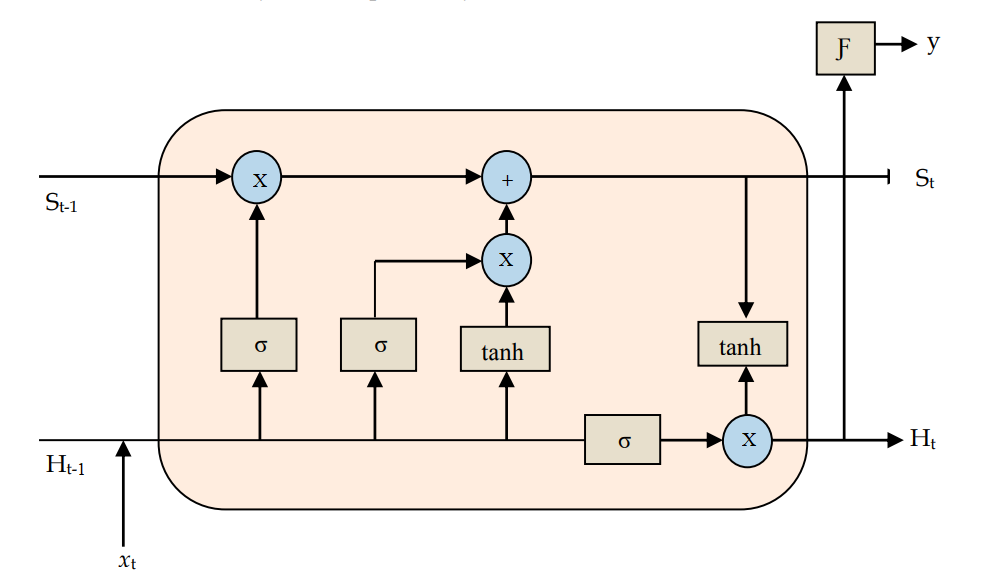
\includegraphics[width=5in]{images/l1.png} 
		\caption{LSTM} %figure name
		\label{LSTM} % for referencing
	\end{center}
\end{figure}
\newpage
\section{Activation Function}
\vspace{-18pt}
The activation function in a neural network is a mathematical function that is applied to a network node's output and decides whether or not the output of the node should be activated based on the weighted total of the inputs. Sigmoid activation function was employed in the project's model.
\subsection{Sigmoid}
\vspace{-18pt}
The main reason why sigmoid function is used because it exists between 0 to 1. Therefore, it is especially used for models where the need is to predict the probability as an output.  Mathematically, Softmax is defined as: 
\begin{eqnarray}
	f(z) = \frac{1}{1 + e^{-z}}
\end{eqnarray}
\section{Binary Cross-Entropy}
\vspace{-18pt}
It is a loss function used in machine learning to measure the difference between predicted binary outcomes and actual binary labels. It quantifies the dissimilarity between probability distributions, aiding model training by penalizing inaccurate predictions. It’s widely used in tasks like binary classification, where the goal is to categorize data into two classes. Binary cross entropy compares each of the predicted probabilities to actual class output which can be either 0 or 1. It then calculates the score that penalizes the probabilities based on the distance from the expected value i.e. how close or far from the actual value.
\section{Adam Optimizer}
\vspace{-18pt}
The Adam optimizer is a popular optimization algorithm used in training deep neural networks. It combines the advantages of two other optimization techniques: AdaGrad and RMSProp. Adam maintains adaptive learning rates for each parameter by calculating an exponentially decaying average of past gradients and their squares. This allows it to dynamically adjust the learning rate for each parameter, typically resulting in faster convergence and better performance compared to traditional optimization algorithms. Adam also includes bias correction to prevent the initial steps from being too large. Overall, Adam is well-suited for a wide range of deep learning tasks due to its efficiency, robustness, and ease of use, often requiring minimal hyper parameter tuning.
\section{Dropout}
\vspace{-18pt}
Dropout is a regularization technique for neural networks, introduced by Geoffrey Hinton, et.al, in 2012. Dropout involves randomly setting a fraction of activation of neurons to 0. This reduces the amount of information available to each layer, forcing the network to learn multiple independent representations of the same data. This makes the network more robust to overfitting. In practice, during each forward pass, each activation in the network is set to zero with a certain probability (e.g., 50\%), effectively dropping out that activation and its corresponding nodes in the network. During the backward pass, the gradients are computed normally and then multiplied by a factor that corresponds to the keep probability. This allows the network to learn to ‘turn on’ different nodes and combinations of nodes to model the data. In a deep neural network architecture, dropout layers are inserted between the dense layers or the convolution layers. The keep probability is typically set to a value between 0.5 and 0.8, depending on the size and complexity of the network and the size of the training data.
\section{Evaluation Metrics}
\vspace{-18pt}
The most important performance indicator (Accuracy, AC) of intrusion detection is used to measure the performance of the model. In addition to the accuracy, we introduce the detection rate and false positive rate. The True Positive (TP) is equivalent to those correctly rejected, and it denotes the number of anomaly records that are identified as anomaly. The False Positive (FP) is the equivalent of incorrectly rejected, and it denotes the number of normal records that are identified as anomaly. The True Negative (TN) is equivalent to those correctly admitted, and it denotes the number of normal records that are identified as normal. The False Negative (FN) is equivalent to those incorrectly admitted, and it denotes the number of anomaly records that are identified as normal.
\begin{table}[tbh]
	\centering
	\begin{tabular}{|c|r|c|} %c,l,r represent alignment, number of c,l or r represent number of columns, | for Vertical line
		\hline %horizontal line
		  &0 &1  \\
		\hline %horizontal line
		0 &TP &FN  \\
		\hline %horizontal line
		1 &FP &TN\\
		\hline
	\end{tabular}
	\caption{Confusion Matrix}
	\label{Confusion Matrix}
\end{table}
\begin{equation}
	Accuracy = \frac{TP + TN}{TP + TN + FP + FN}
\end{equation} 
Precision is the number of actual attacks as a proportion of the number classified as attacks.
\begin{equation}
	Precision = \frac{TP}{TP + FP} 
\end{equation}
True Positive Rate or Recall shows the percentage of the number of records identified correctly over the total number of anomaly records.
\begin{equation}
	True Positive Rate/ Recall = \frac{TP}{FN + TP}
\end{equation}
False Positive Rate is the percentage of the number of records rejected incorrectly is divided by the total number of normal records.
\begin{equation}
	False Positive Rate = \frac{FP}{FP + TN}
\end{equation}
The F1 Score is the weighted average of Precision and Recall. Therefore, this score takes both false positives and false negatives into account.
\begin{equation}
	F1 Score = \frac{2 * Precision * Recall}{Precision + Recall}
\end{equation}
\section{Software Defined Networking}
\vspace{-18pt}
Software-Defined Networking (SDN) is a revolutionary network architecture approach that decouples the control plane from the data plane in traditional networking models. By centralizing control functions in a software-based controller, SDN enables dynamic management and programmability of network resources. This separation allows administrators to orchestrate network behaviour centrally, facilitating rapid provisioning, configuration, and optimization of network services. SDN simplifies network management by abstracting underlying infrastructure complexities and providing a unified interface for network automation and orchestration. Through programmable interfaces and open standards like OpenFlow, SDN empowers organizations to tailor network behaviour to specific application requirements, enhance agility, and support innovative network services.
\section{Mininet}
\vspace{-18pt}
Mininet is an open-source software emulation platform for creating virtual networks. It allows users to create a realistic network topology on a single machine for testing, research, and educational purposes. Mininet provides a lightweight and easy-to-use environment for experimenting with SDN (Software-Defined Networking) concepts without the need for physical networking hardware. Mininet allows users to define custom network topologies using a simple Python-based API. Users can specify the number and types of nodes (switches, routers, hosts), the links between them, and even customize parameters such as bandwidth, delay, and loss rates. Mininet utilizes Linux container (LXC) technology to create lightweight virtual network devices. Each network element (node) in a Mininet topology runs as a separate process inside a Linux container, providing isolation and efficient resource utilization. Mininet supports integration with various SDN controllers, including OpenDaylight, ONOS, Ryu, POX, and others. Users can choose their preferred SDN controller and configure Mininet to connect to it, enabling experimentation with different controller functionalities and SDN applications.
\section{POX Controller}
\vspace{-18pt}
POX Controller is an open-source software-defined networking (SDN) controller framework developed in Python. As a controller, it serves as the centralized brain of an SDN network, managing and orchestrating the flow of data traffic within the network. POX Controller enables network administrators to dynamically control and configure network devices, such as switches and routers, by providing a programmable interface for implementing network policies and forwarding rules. Built on the event-driven architecture of Python, POX Controller offers flexibility and extensibility, allowing users to develop custom network applications and services tailored to their specific requirements. It supports various SDN protocols, including OpenFlow, enabling seamless integration with SDN-enabled devices.
\section{Wireshark}
\vspace{-18pt}
Wireshark is a powerful open-source network protocol analyser that allows users to capture, analyse, and interpret network traffic in real-time or from previously captured data. With its intuitive user interface and extensive protocol support, Wireshark enables users to inspect packets at a granular level, dissecting each one to reveal details such as source and destination addresses, protocols used, packet contents, and timing information. This level of visibility makes Wireshark invaluable for network troubleshooting, as it helps identify and diagnose issues such as connectivity problems, performance bottlenecks, and security threats. Additionally, Wireshark provides advanced features such as customizable display filters, statistical analysis tools, and packet reconstruction capabilities, empowering users to efficiently analyse network behaviour, detect anomalies, and optimize network performance.
\section{CICFlowMeter}
\vspace{-18pt}
CICflowmeter or the Canadian Institute for Cybersecurity Flow Meter, is a network traffic analysis tool designed to monitor and analyse network flows, providing insights into network behaviour and traffic patterns. Specifically tailored for cybersecurity purposes, CICflowmeter focuses on detecting and analysing network flows related to cyber threats, such as malicious activities, attacks, and anomalies. By capturing and dissecting flow data, including source and destination IP addresses, ports, protocols, and packet sizes, CICflowmeter offers detailed visibility into network traffic, allowing security analysts to identify potential security breaches, intrusions, or suspicious behaviour.
\section{Probe}
\vspace{-18pt}
A probe attack is a reconnaissance technique used by attackers to gather information about a target system, network, or infrastructure. The term "probe" refers to the act of probing or investigating the target to identify vulnerabilities, weaknesses, or potential points of entry for further exploitation. The primary objective of a probe attack is to gather information about the target environment without directly causing any damage or disruption. Attackers aim to identify potential security weaknesses that can be exploited in subsequent stages of an attack. Probe attacks typically involve reconnaissance activities where the attacker gathers information about the target. This information can include network topology, system configurations, installed software and services, open ports, and potential entry points into the network.
\section{DDoS}
\vspace{-18pt}
A Distributed Denial of Service (DDoS) attack is a malicious attempt to disrupt the normal traffic of a targeted server, service, or network by overwhelming it with a flood of internet traffic. Unlike traditional Denial of Service (DoS) attacks, where a single source is used to flood the target, DDoS attacks involve multiple sources, often tens of thousands or more, distributed across the internet. The primary goal of a DDoS attack is to render a targeted system, network, or service unavailable to its users by overwhelming it with a massive volume of traffic. This disrupts the normal operation of the target, causing it to become slow, unresponsive, or completely unavailable. DDoS attacks are executed by a network of compromised devices, often referred to as a botnet. These devices can include computers, servers, Internet of Things (IoT) devices, routers, and even smartphones infected with malware. The attacker gains control of these devices by infecting them with malicious software, such as viruses, worms, or Trojans, turning them into "bots" or "zombies" that can be remotely controlled. Once the botnet is established, the attacker instructs the compromised devices to flood the target with a massive volume of traffic. This flood of traffic overwhelms the target's resources, making it unable to respond to legitimate user requests.
\chapter{Methodology}
\section{Working Mechanism}
\vspace{-18pt}
The development of Network Intrusion Detection System involves major steps which is 
depicted in the diagram given below:
\begin{figure}[tbh] % tbh means top, bottom or here (priority: left to right)
\begin{center}
	%
\includegraphics[width = 3in]{images/logo.png}
	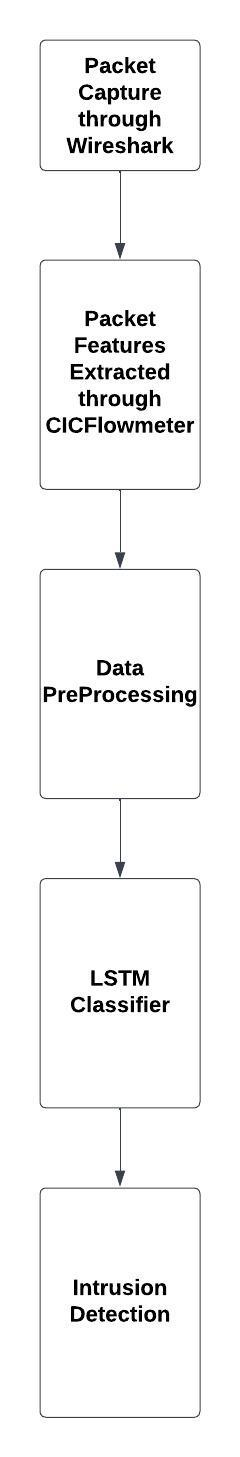
\includegraphics[width=1in]{images/workMan.jpg} 
	\caption{Working mechanism of Network Intrusion Detection System} %figure name
	\label{Working mechanism of Network Intrusion Detection System} % for referencing
\end{center}
\end{figure}
\subsection{Packet Capture through Wireshark}
\vspace{-18pt}
To capture packets from Wireshark, we should first select the network interface from which we want to capture packets. After selecting the capture interface, we can start the capture session. Wireshark begins capturing packets from the chosen interface and displays them in real-time in the main capture window. We can stop the packet capture session at any time by clicking the "Stop" button in Wireshark's capture toolbar. Once the capture is stopped, we can save the packet records in a .pcap extension file.
\subsection{Data set}
\vspace{-18pt}
InSDN is a comprehensive Software-Defined Network dataset for Intrusion detection system evaluation. The new dataset includes the benign and various attack categories  that can occur in different elements of the SDN standard. InSDN considers different attack, including DoS, DDoS, brute force attack, web applications, exploitation, probe, and botnet. Furthermore, the normal traffic in the generated data covers  various  popular  application services such as HTTPS, HTTP, SSL, DNS, Email, FTP, SSH, etc. The dataset was generated by using four virtual machines (VMs). The first virtual machine is a Kali Linux one and represents the attacker server. The secondary machine is a Ubuntu 16.4 one, and acts on the ONOS controller. Third is an Ubuntu 16.4 machine to serve for the Mininet and OVS switch. The forth virtual machine is a Linux one based on metasploitable-2 to provide vulnerable services for demonstrating common vulnerabilities.\cite{article}
\begin{figure}[h] % tbh means top, bottom or here (priority: left to right)
\begin{center}
	%
\includegraphics[width = 3in]{images/logo.png}
	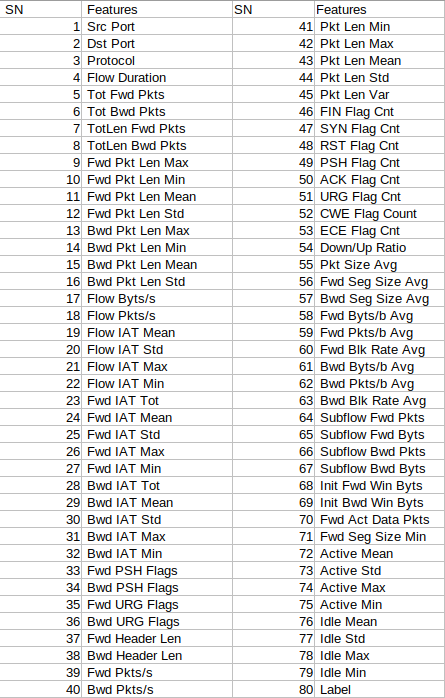
\includegraphics[width=4in]{images/ds2.png} 
	\caption{Features of InSDN dataset} %figure name
	\label{} % for referencing
\end{center}
\end{figure}
\subsection{Packet Features Extracted through CICflowmeter}
\vspace{-18pt}
The CICflowmeter takes the .pcap extension file and extracts 80 network traffic analysis features which are the same as the features of the InSDN dataset except for the label column.
\subsection{Data Preprocessing}
\vspace{-18pt}
We used the InSDN datasets and first dropped some label values in the Label column. The label values that were dropped from the dataset were U2R, BFA and DoS. Then we dropped columns like Timestamp, Flow\_ID, Src\_IP and Dst\_IP before the normalization step. For the efficient training of neural networks, the numeric input data should be transformed by performing some pre-processing known as data normalization. It is used where inputs are widely divergent. Without such a process, networks would take a long time to train. Different schemes can be used to normalize the input data before it is fed to the input layer of neural network. We used Min-Max normalization to normalize the attributes of our dataset. Min-max normalization is one of the most common ways to normalize data. For every feature, the minimum value of that feature gets transformed into a 0, the maximum value gets transformed into a 1, and every other value gets transformed into a decimal between 0 and 1. Mathematically,
\begin{equation}
x' = \frac{x- min(x)}{max(x)-min(x)}
\end{equation}
where $x: $ Original value,\\ $max(x): $ Maximum value of x,\\ $min(x): $ Minimum value of x and \\ 
$x': $ Normalised value. \par 
For the label column in the dataset, we used Label encoding to convert the string values into numerical ones so as to fit in the LSTM model. 
\subsection{Feature Extraction}
\vspace{-18pt}
Random Forest Classifier, or RFC, is an ensemble learning method that creates a forest of decision trees, where each tree is trained on a random subset of the data, and a random subset of the features. It provides a feature importance score based on how much each feature reduces impurity across all decision trees in the forest. Recursive Feature Elimination, or RFE is a feature selection technique that recursively fits a model and removes the least important features until the desired number of features is reached. It works by repeatedly training the model, ranking the features based on their importance, and removing the least important features. It is particularly useful when the number of features is large, as it helps to reduce the complexity of the model and improves its interpretability.
Algorithm for RFC with RFE is given as:
\begin{enumerate}[label=\roman*.]
\item Initialise the Random Forest Classifier with the required number of trees.
\item Use RFE for feature selection taking parameters like RFC as the base estimator and number of features to select.
\item Fit RFE to the training datasets.
\item Get the boolean masks of the selected features from RFE.
\item Extract the names of the selected features.
\item Create a new data frame containing the selected features.
\end{enumerate}
\subsection{LSTM Architecture}
\vspace{-18pt}
\begin{figure}[tbh]
	\begin{center}
		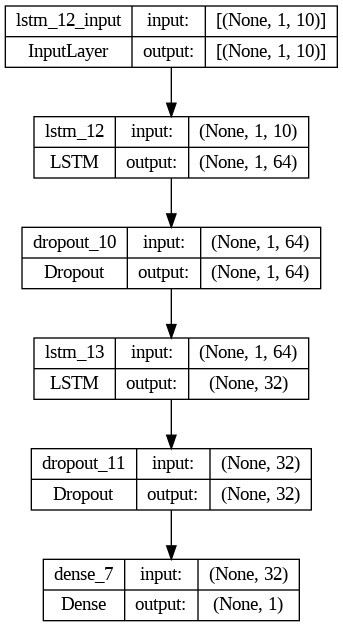
\includegraphics[width=2in]{images/lstm_Model.png}
		\caption{LSTM model}
		\label{LSTM model}
	\end{center}
\end{figure}
\newpage
The block diagram shows the layers used in the trained LSTM model.
\begin{enumerate}[label=\roman*.]
	\item LSTM layer: This is the core layer of the model. It is responsible for learning long-term dependencies in the input data. It consists of cells that store information and gates that control the flow of information into and out of the cells.
	\item Dropout layer: This layer is a regularization technique used to prevent the model from overfitting on the training data.
	\item Dense layer: This is the layer responsible for mapping the output of the LSTM layers to a final output. 
\end{enumerate}
In our model as we can see from the figure, the input to the LSTM model has dimensions of (None,1,10) which is due to the reshaping of the train and test datas done before passing it as a parameter to the model. The number 10 signifies the number of best features that we selected from the original dataset. The output from this first layer is fed into the second layer with different number of neuron after passing it through the dropout layer in between the two layers. The final dense layer has one neuron and outputs a single value. This model that we have trained is being used for binary classification task where the output is a single value that indicates whether the input is a type of attack or not.\par 
The same model will then be used to classify the label of attacks in the next step of our predictions. If the traffic is classified as a type of attack by our first model, then the second model will then check to correctly predict the label of our attack traffic. This model also outputs a single value that maps to either a DDoS traffic or a Probe traffic.
\section{Model Training and Optimization}
\vspace{-18pt}
\subsection{Model Training Algorithm}
\vspace{-18pt}
\begin{enumerate}[label=\roman*.]
	\item Import the required libraries for data preprocessing including numpy, pandas and scikit-learn.
	\item Normalise the dataset and label encode the Label column.
	\item Using the train-test split function, divide the datasets into training and testing datasets in an 8:2 ratio.
	\item Reshape the train and test set to then pass it as a input parameter for the LSTM model.
	\item Compile the model using Adam optimizer using an appropriate learning rate, loss function of binary crossentropy and use accuracy as the metric.
	\item Fit the model on the training using the fit() function of the model. Save the object returned by the function in a history parameter.
	\item  Plot for training and validation loss against number of epochs.
\end{enumerate}
\subsection{Model Deployment Algorithm}
\vspace{-18pt}
\begin{enumerate}[label=\roman*.]
	\item Save the trained models to a keras file format. 
	\item Load the trained models into the system for validation.
	\item Test the trained models on unseen network traffic and verify its performance.
	\item Load the model into the Tkinter application.
\end{enumerate}
\section{System Diagram}
\vspace{-18pt}
\subsection{Use case diagram}
\begin{figure}[h]
\begin{center}
	%
\includegraphics[width = 3in]{images/logo.png}
	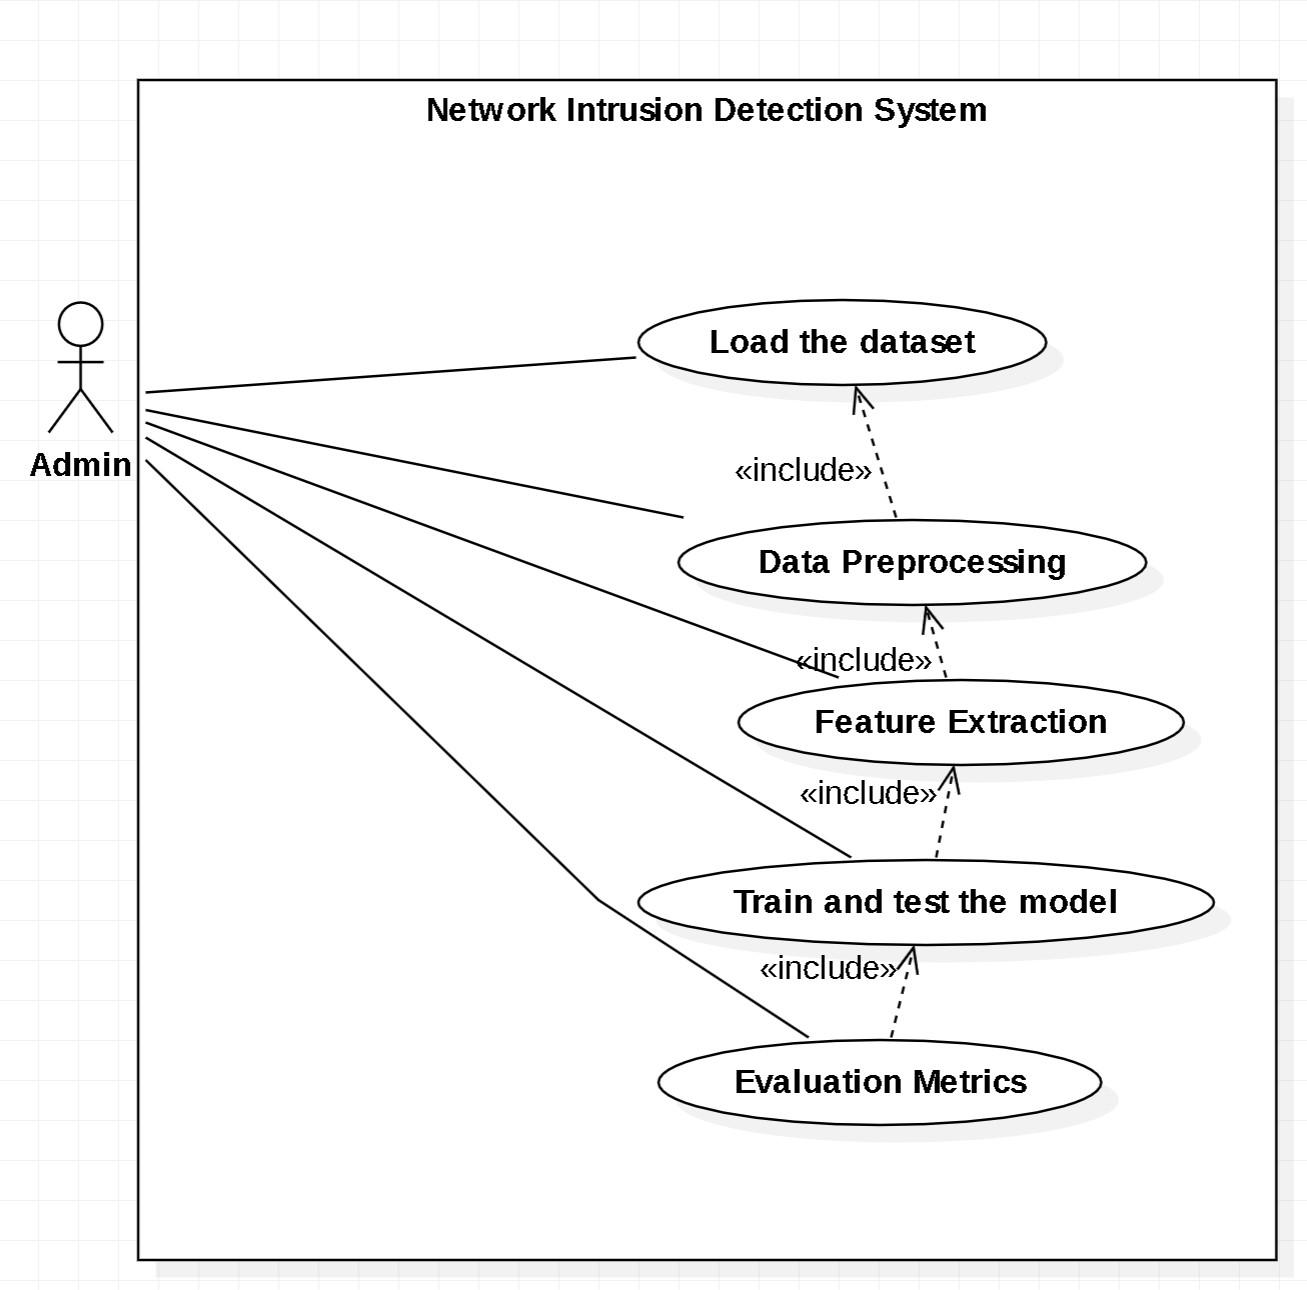
\includegraphics[width=5in]{images/use.jpg} 
	\caption{Use case Diagram of Network Intrusion Detection System} %figure name
	\label{Use case Diagram of Network Intrusion Detection System} % for referencing
\end{center}
\end{figure}
\newpage
\subsection{Simulation Environment}
\vspace{-18pt}
The simulation was created in a virtual machine (Orcale VM VirtualBox) using Ubuntu-22.04.3 as Mininet only support Linux OS. The architecture of our network composes of two virtual switch namely s1 and s2, pox controller c0, Mininet virtual host namely h1, h2, h3, h4, h5 and h6. The virtual switch s1 is connected to Mininet virtual host h1, h2 and h3. The virtual switch s2 is connected to Mininet virtual host h4, h5 and h6. The communication between all virtual hosts is done by L2 connectivity. The legitimate network traffic was generated through Linux machine (Ubuntu-22.04.3) which is connected to the Internet. The DDoS Traffic was generated through Mininet virtual host using hping3 tool. The Probe Traffic was generated through Mininet virtual host using Nmap tool.\par 

\begin{figure}[tbh]
	\begin{center}
		%
\includegraphics[width = 3in]{images/logo.png}
		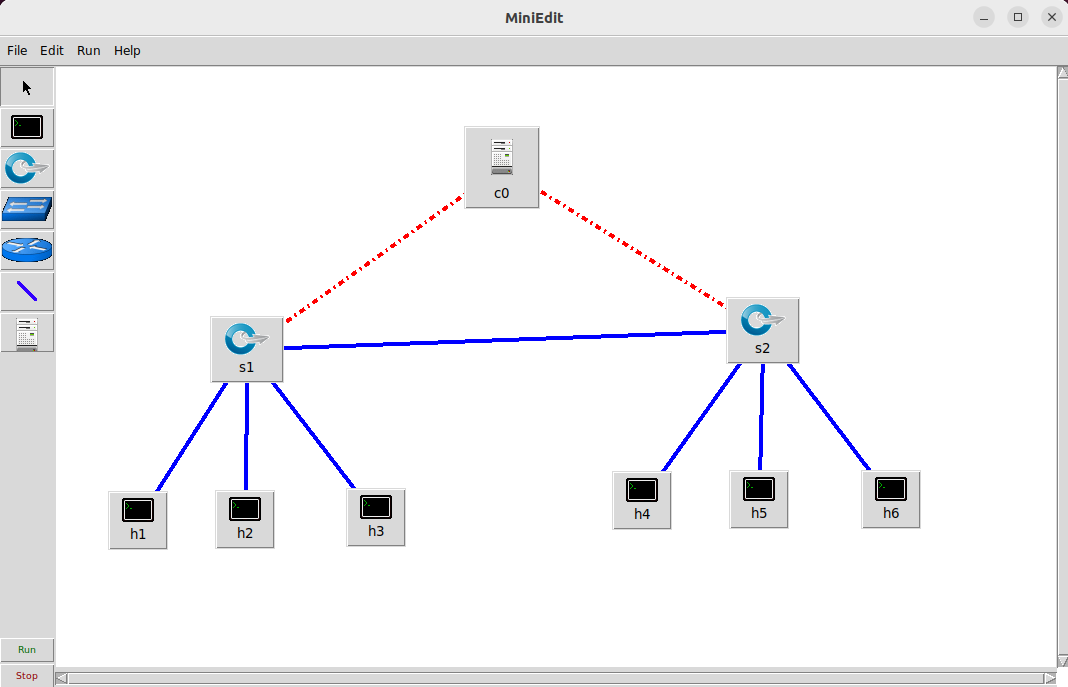
\includegraphics[width=5in]{images/simenv.png} 
		\caption{Simulation Environment} %figure name
		\label{Simulation Environment} % for referencing
	\end{center}
\end{figure}
\subsection{Software Development Model}
\vspace{-18pt}
Incremental model is a method of software engineering that combines the elements of waterfall model in iterative manner. It involves both development and maintenance. In this model requirements are broken down into multiple modules. Incremental development is done in steps from analysis design, implementation, testing/verification, maintenance. Each iteration passes through the requirements, design, coding and testing phases. The first increment is often a core product where the necessary requirements are addressed, and the extra features are added in the next increments. The core product is delivered to the client. Once the core product is analyzed by the client, there is plan development for the next increment.\par
\begin{figure}[tbh] % tbh means top, bottom or here (priority: left to right)
	\begin{center}
		%
\includegraphics[width = 3in]{images/logo.png}
		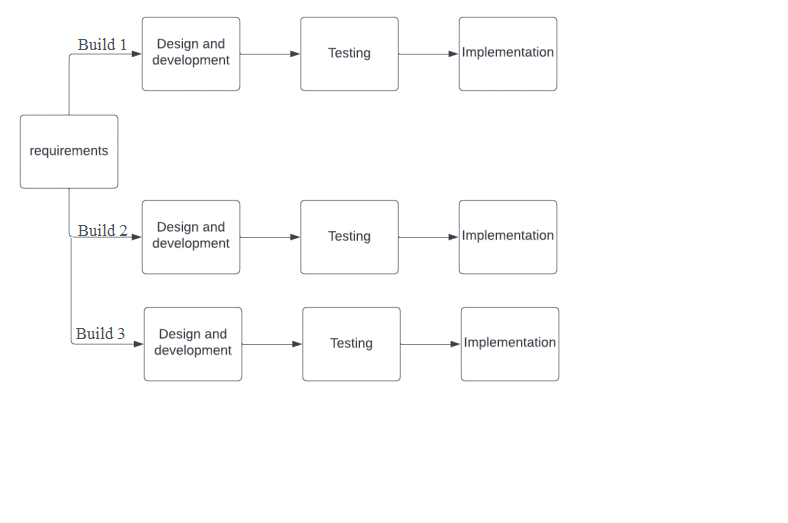
\includegraphics[width=6in]{images/sdlc1.png} 
		\caption{Incremental Model} %figure name
		\label{Incremental Model} % for referencing
	\end{center}
\end{figure}
\begin{itemize}
	\item First build: The feature extraction process was done where features were reduced from 81 to 10 and demo model was built.
	\item Second build: The model was optimized and validated through test data.
	\item Third build: The model was tested with real world traffic and integrated with SDN.
\end{itemize}
\chapter{Results and Discussion}
\vspace{-18pt}
The project takes in various parameters and then provides the user with the most probable label for the respective inputs. Before training the model, we loaded the required datasets and performed necessary preprocessing steps. The feature extraction was done via Random Forest Classifier where we selected the top 10 features from the dataset. For training the LSTM model, we first reshaped the input shapes to pass it as an input to the model. We label encoded the values in the Label columns. The loss plot that we have calculated on the training and test dataset is to determine the model's training efficiency. The LSTM models that we designed takes in the parameters and trains upto the required number of epochs.  \par 
\begin{figure}[tbh]
	\begin{center}
		%
\includegraphics[width = 3in]{images/logo.png}
		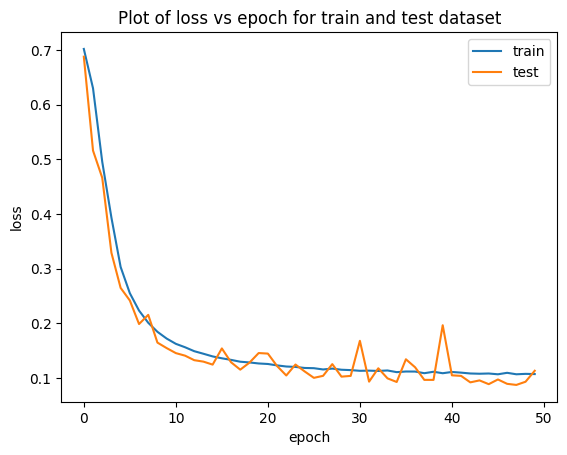
\includegraphics[width=4in]{images/normalvovs.png} 
		\caption{Loss plot of Normal and Attack labels for train and test dataset} %figure name
		\label{Loss plot of Normal and Attack labels for train and test dataset} % for referencing
	\end{center}
\end{figure}
\begin{figure}[tbh]
	\begin{center}
		%
\includegraphics[width = 3in]{images/logo.png}
		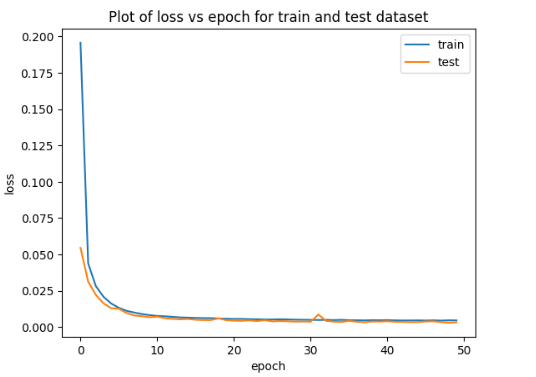
\includegraphics[width=4in]{images/attloss.png} 
		\caption{Loss plot of Normal and Attack labels for train and test dataset} %figure name
		\label{Loss plot for train and test dataset} % for referencing
	\end{center}
\end{figure}
We divided the original dataset into train and test set with 80/20 split. We then trained the LSTM models for the train set and checked the confusion matrix for both the test set and the validation set that we created, for both binary classifications. The first LSTM model helps distinguish between attacks and normal traffic. If the traffic is classified as an attack by the first model, the second LSTM model then checks for the label of the attack(DDoS or Probe) to predict the correct class.\par
 \begin{figure}[tbh] % tbh means top, bottom or here (priority: left to right)
	\begin{center}
		%
\includegraphics[width = 3in]{images/logo.png}
		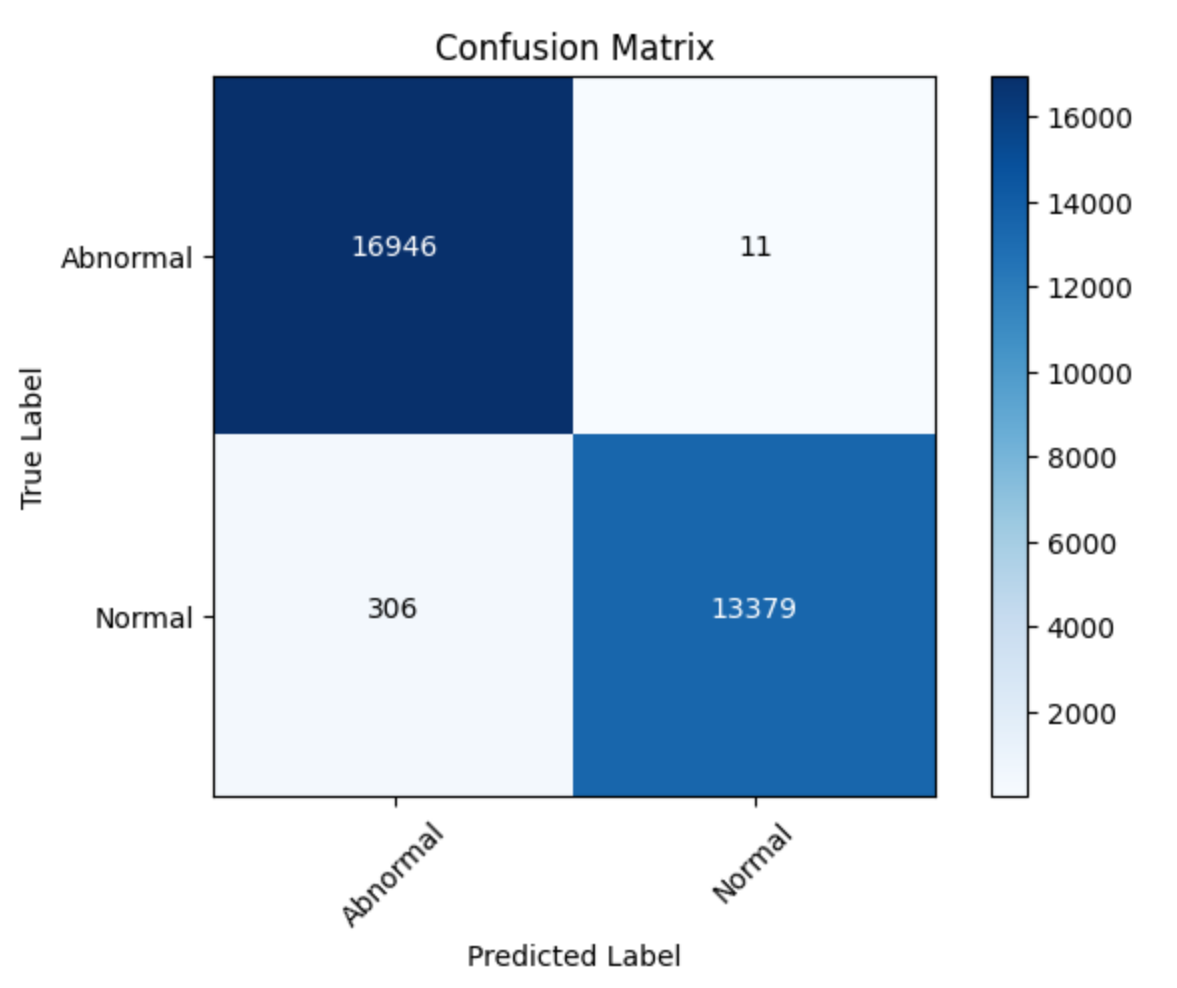
\includegraphics[width=4in]{images/testmat.png} 
		\caption{Confusion Matrix of Normal and Attack labels for Test dataset} %figure name
		\label{Confusion Matrix of Normal and Attack labels for Test dataset} 
	\end{center}
\end{figure}
\begin{table}[tbh]
	\centering
	\begin{tabular}{|c|r|c|l|} %c,l,r represent alignment, number of c,l or r represent number of columns, | for Vertical line
		\hline %horizontal line
		Label  &Precision &Recall &F1-score \\
		\hline %horizontal line
		Abnormal &0.98 &1.00 &0.99 \\
		\hline %horizontal line
		Normal &1.00 &0.98 &0.99\\
		\hline
	\end{tabular}
	\caption{Evaluation Metrics of Normal and Attack labels for Test dataset}
	\label{Evaluation Metrics of Normal and Attack labels for test dataset}
\end{table}
 \begin{figure}[tbh] % tbh means top, bottom or here (priority: left to right)
 	\begin{center}
 		%
\includegraphics[width = 3in]{images/logo.png}
 		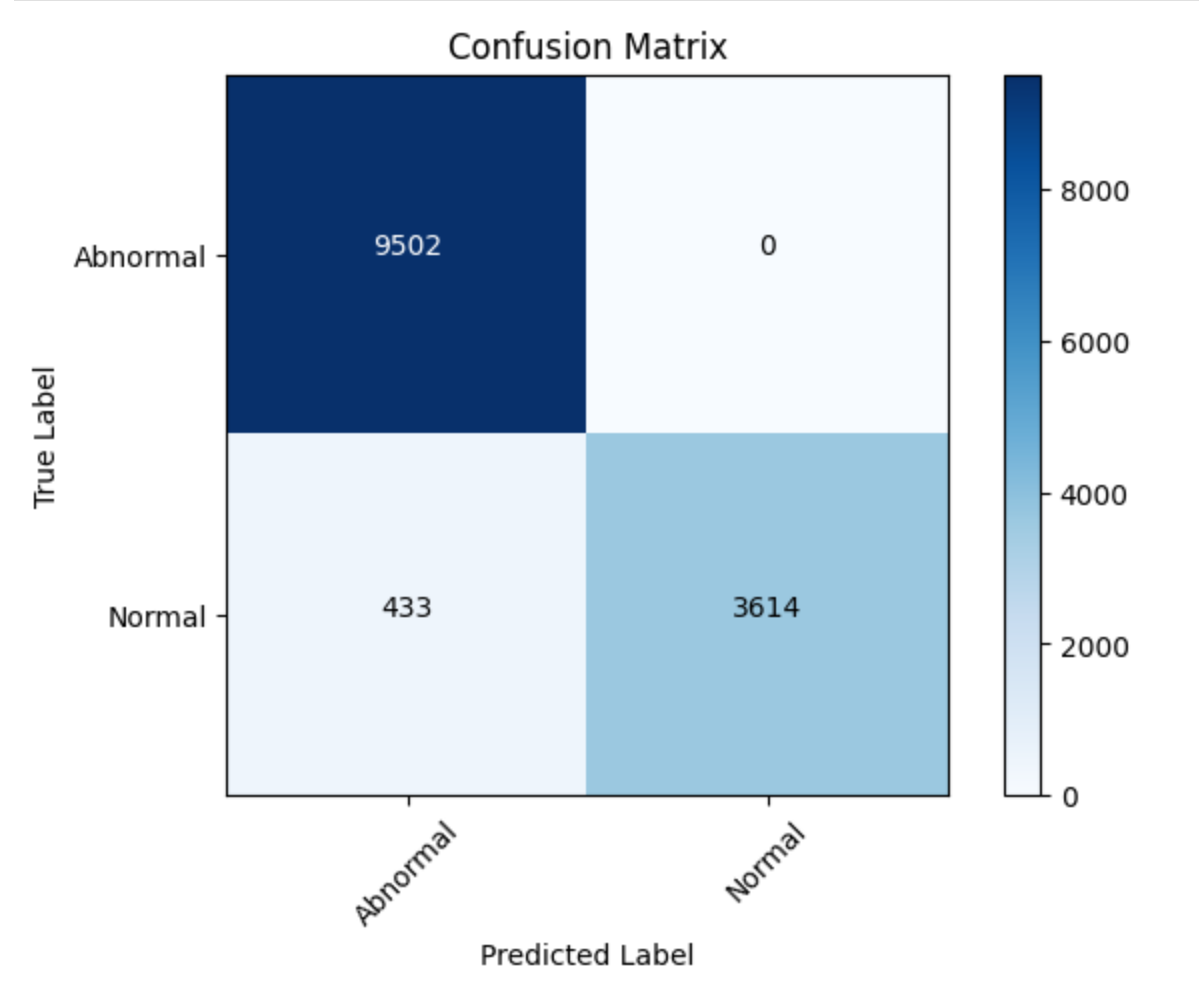
\includegraphics[width=4in]{images/confMatnormvatt.png} 
 		\caption{Confusion Matrix of Normal and Attack labels for Validation dataset} %figure name
 		\label{Confusion Matrix of Normal and Attack labels for Validation dataset} 
 	\end{center}
 \end{figure}
For the Normal and Abnormal traffics, the confusion matrix for the validation test tells us the following:\\ 
True Positive(TP) : 9502. These are the traffics that were correctly identified as attacks.\\
False Positive(FP): 433. These are the datas that were incorrectly identified as attacks.\\
False Negative(FN): 0. No datas were incorrectly identified as Normal label.\\
True Negative(TN): 3614. These datas are correctly identified as Normal traffic.\\

\begin{table}[tbh]
	\centering
	\begin{tabular}{|c|r|c|l|} %c,l,r represent alignment, number of c,l or r represent number of columns, | for Vertical line
		\hline %horizontal line
		Label  &Precision &Recall &F1-score \\
		\hline %horizontal line
		Abnormal &0.96 &1.00 &0.98 \\
		\hline %horizontal line
		Normal &1.00 &0.89 &0.94\\
		\hline
	\end{tabular}
	\caption{Evaluation Metrics of Normal and Attack labels for Validation dataset}
	\label{Evaluation Metrics of Normal and Attack labels for validation dataset}
\end{table}
For the Abnormal traffics, the confusion matrix for the validation test tells us the following:\\ 
True Positive(TP) : 3042. These are the traffics that were correctly identified as DDoS attacks.\\
False Positive(FP): 8. These are the datas that were incorrectly identified as DDoS attacks.\\
False Negative(FN): 1458. These datas were incorrectly identified as Probe label.\\
True Negative(TN): 4994. These datas are correctly identified as Probe traffic.\par 
\begin{figure}[tbh] % tbh means top, bottom or here (priority: left to right)
	\begin{center}
		%
\includegraphics[width = 3in]{images/logo.png}
		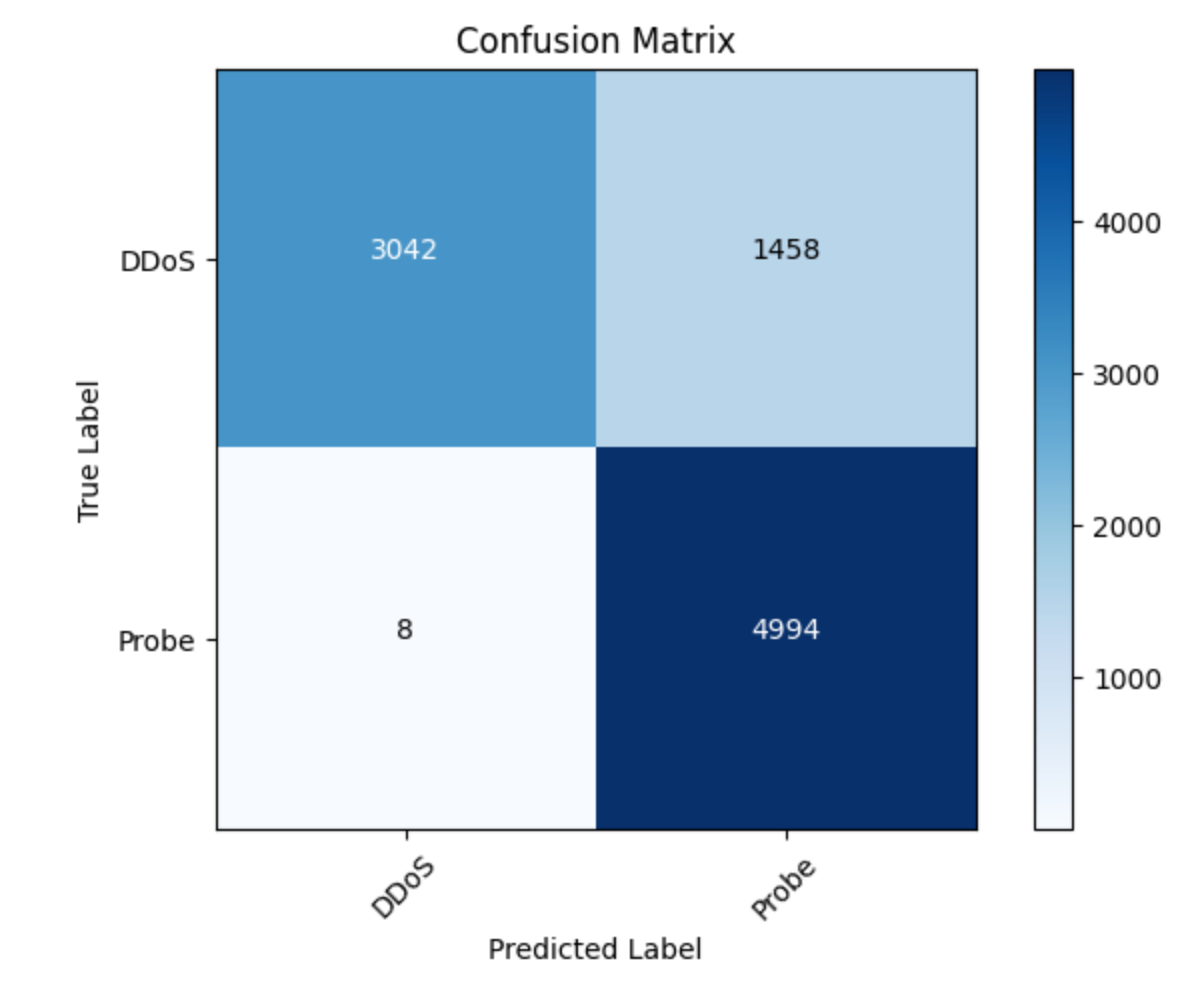
\includegraphics[width=4in]{images/valattacksmat.png} 
		\caption{Confusion Matrix of Attack labels for Validation dataset} %figure name
		\label{Confusion Matrix of Attack labels for Validation dataset} 
	\end{center}
\end{figure}
\begin{table}[tbh]
	\centering
	\begin{tabular}{|c|r|c|l|} %c,l,r represent alignment, number of c,l or r represent number of columns, | for Vertical line
		\hline %horizontal line
		Label  &Precision &Recall &F1-score\\
		\hline %horizontal line
		DDoS &1.00 &0.68 &0.81\\
		\hline %horizontal line
		Probe &0.77 &1.00 &0.87\\
		\hline
	\end{tabular}
	\caption{Evaluation Metrics of Attack labels for Validation dataset}
	\label{Evaluation Metrics of Attack labels for validation dataset}
\end{table}
From the figures obtained from the evaluation on test and validation sets, we can see that our model achieves satisfying results on the input data. \par
\begin{table}[tbh]
	\centering
	\begin{tabular}{|c|r|c|} %c,l,r represent alignment, number of c,l or r represent number of columns, | for Vertical line
		\hline %horizontal line
		  &Model 1 &Model 2 \\
		\hline %horizontal line
		Test set &0.99 &0.97 \\
		\hline %horizontal line
		Validation set &blank &0.85 \\
		\hline
	\end{tabular}
	\caption{Comparison of accuracy}
	\label{Accuracy comparison}
\end{table}
The False Positive rate in test dataset for normal and attack classification was measured as 0.0224 whereas it was 0.106 in the validation dataset. Similarly for the attack labels in validation dataset we obtained 0.0015 as False Positive rate which is a very promising number.
\chapter{Conclusion}
\vspace{-18pt}
\section{Limitations}
\vspace{-18pt}
\begin{enumerate}[label=\roman*.]
	\item Our system can only detect DDoS, Normal and Probe traffics.
	\item Our system is only 97\% accurate for binary classification for normal and attack labels and only 85\% accurate in predicting the correct attack label in real world traffic.
	\item Our system cannot perform real time monitoring.
\end{enumerate}
\section{Future Enhancements}
\vspace{-18pt}
Additional dataset containing more variety of attacks can be added and used to train the model to increase the accuracy as well as to detect more variety of attacks. Our system works on batch processing. This can be changed into a real time monitoring system by doing a packet feature extraction through the system itself rather than using CICflowmeter and Wireshark.
\section{Conclusion}
\vspace{-18pt}
Therefore in this project, we developed a Network Intrusion Detection System which is capable of detecting attacks in a computer network. The features were reduced from original 81 features to 10 features  by using Random Forest Algorithm. We used the InSDN dataset for our assessments and obtained promising results to reach our objective. Our project seeks to develop a robust system that can effectively detect the intrusions within a computer network.
\newpage
%Reference
\renewcommand\bibname{References} % Change heading to References
\bibliographystyle{IEEEtran} % to use IEEE Format for referencing
\addcontentsline{toc}{chapter}{References} % to add references in TOC
\bibliography{library} % specify the .bib file containing reference information 

\chapter*{Appendix}
\addcontentsline{toc}{chapter}{Appendix}
\begin{figure}[tbh]
	\begin{center}
		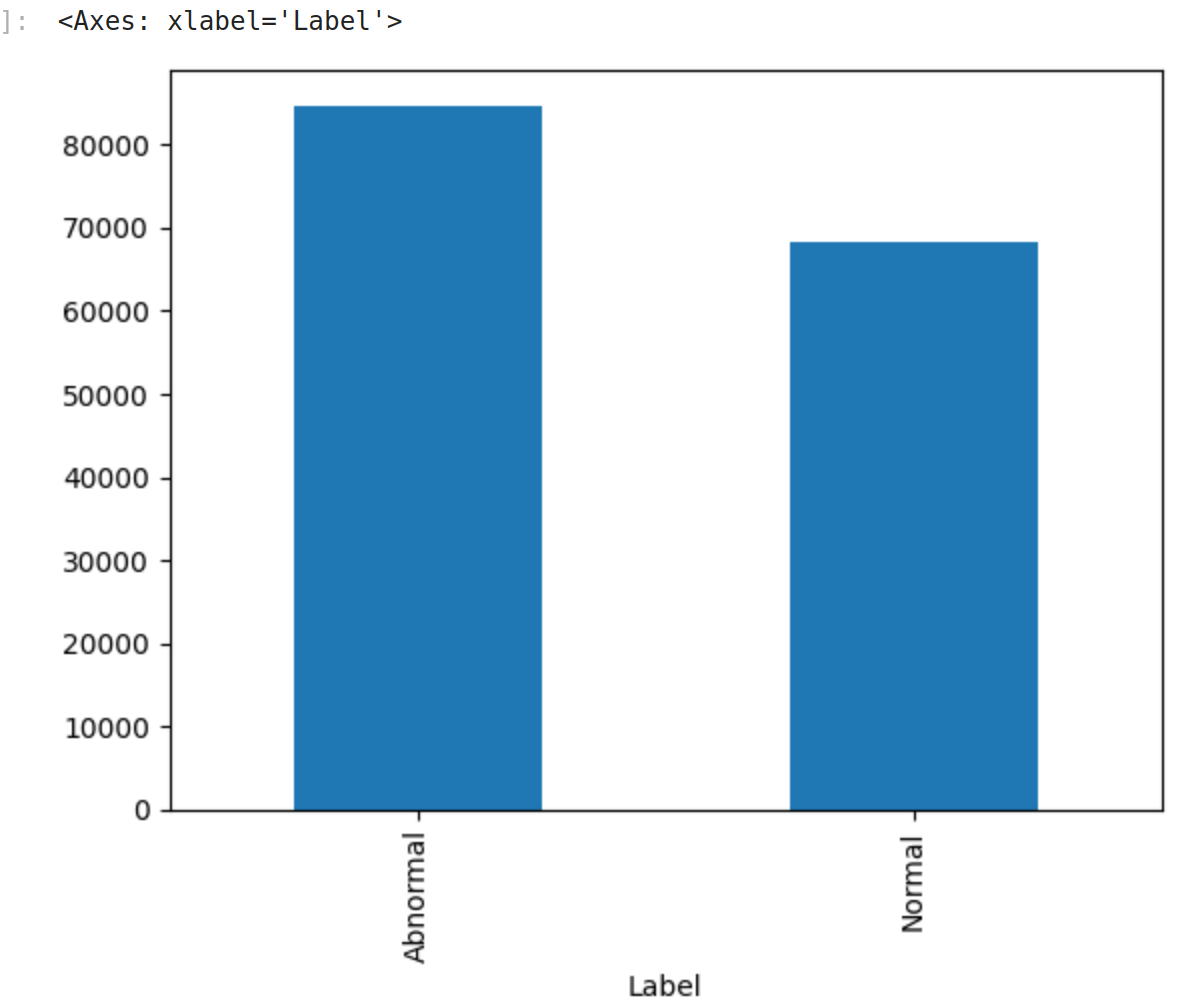
\includegraphics[width=4in]{images/binvattlab.png}
	\end{center}
\end{figure}
\begin{figure}[tbh]
	\begin{center}
		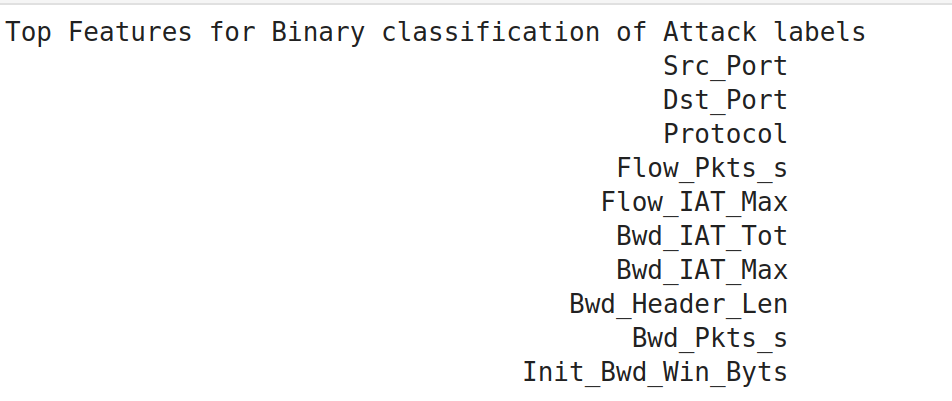
\includegraphics[width=5in]{images/attlab.png}
	\end{center}
\end{figure}
\begin{figure}[tbh]
	\begin{center}
		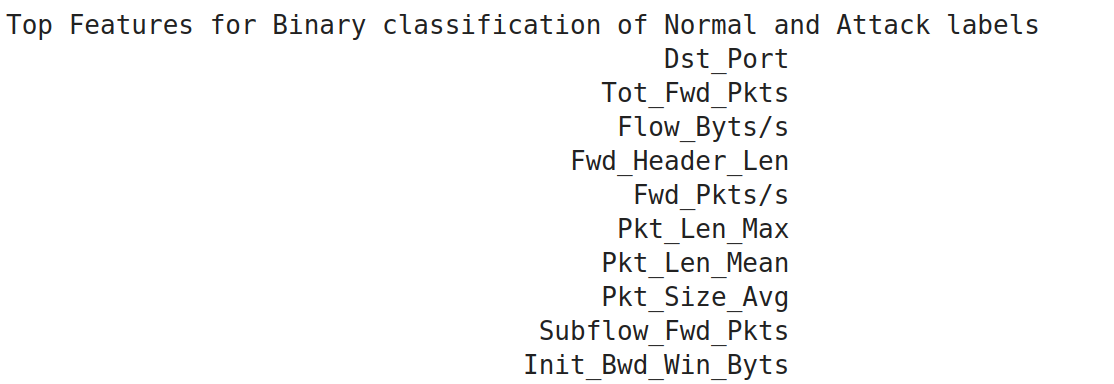
\includegraphics[width=6in]{images/top10normatt.png}
	\end{center}
\end{figure}
\chapter*{Annex}
\addcontentsline{toc}{chapter}{Annex}
\begin{figure}[tbh]
	\begin{center}
		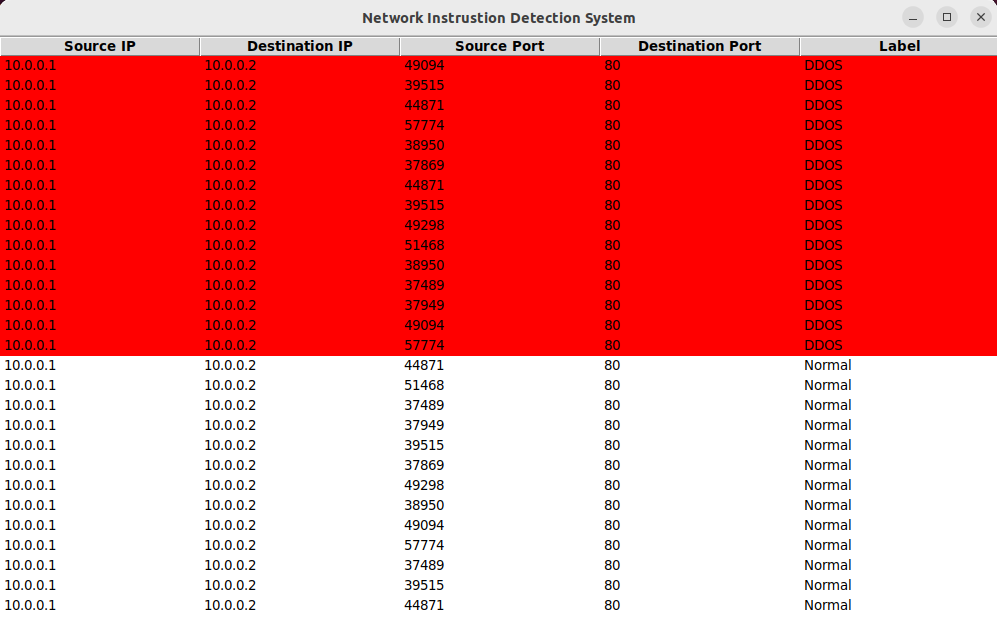
\includegraphics[width=5in]{images/annex.png}
	\end{center}
\end{figure}
%\chapter*{brother}
%\addcontentsline{toc}{chapter}{bro}
\end{document}
